\documentclass[11pt,letterpaper]{article}
\usepackage{array}
\usepackage{fullpage}
\usepackage{graphicx}
\usepackage{parskip}
\usepackage{amsmath}
\usepackage[small]{caption}
\usepackage{graphpap}
\usepackage{logpap}
\usepackage{tabularx}
\usepackage{url}
\usepackage{hyperref}
\usepackage{enumitem}

\renewcommand{\thesection}{PART \arabic{section}: }

\newcounter{question}[section]
\newenvironment{question}[1][]{\refstepcounter{question}\par\medskip
   \textbf{\arabic{section}.\thequestion.} \rmfamily}{\medskip}

\usepackage{titlesec}
\titleformat{\section}{\clearpage\normalfont\bfseries}{\thesection}{0em}{}
\titlespacing{\section}{0pt}{0.5\baselineskip}{0pt}

\titleformat{\subsection}[runin]
{\normalfont\bfseries}{\thesubsection}{1em}{}

\titleformat{\subsubsection}{\normalfont\bfseries}{\thesubsubsection}{0em}{}
\titlespacing{\subsubsection}{0pt}{0.5\baselineskip}{0pt}

\newcounter{saveenumi}
\newcommand{\seti}{\setcounter{saveenumi}{\value{enumi}}}
\newcommand{\conti}{\setcounter{enumi}{\value{saveenumi}}}

\usepackage[dvipsnames]{xcolor}
\newcommand{\sol}[1]{{\color{NavyBlue} #1}}


\begin{document}
\setlength{\parindent}{0in}

%% EQUIP: Force Probe, Pulley, Track, Hangar, Weight, Tilt, Scale

\begin{flushright}
PHYS S211: General Physics I\\
Lab 6: Statics\\
10/15/24 (due 10/22/24)
\end{flushright}

Name(s):\\

\subsubsection*{Topics:}
\begin{enumerate}
\setlength{\parskip}{3pt}
\item Torque / torque balance
\item Static equilibrium
\end{enumerate}

\subsubsection*{Introduction:}
In this lab you will test the relationships between force, torque, and static equilibrium by performing a series of experiments in which masses are hung from a meter stick. Recall that when a system is in equilibrium,
$$\sum{F_x}=0$$
$$\sum{F_y}=0$$
$$\sum\tau=0$$

\subsubsection*{What you should turn in:} 
You may submit a group report. Submit the report as a single document and clearly indicate if you are submitting it as a group report. 

\begin{itemize}
\setlength{\parskip}{3pt}
\item Part 1: Graph of position vs. 1/weight and best-fit line through the data. [3 pts]
\item Part 1: Theoretical relationship between position and weight, and discussion of how it compares to your observations. [3 pts]
\item Part 2a: Calculation of the mass of the meter stick, including derivation that shows how you made the calculation. [3 pts]
\item Part 2b: Comparison of distance in unequal arm balance to theoretical values, including derivation. [3 pts]
\item Part 3: Determination of mass of the hanging sphere by using the tension protractors. [3 pts]
\item Part 3: Calculation of initial angular acceleration and response to questions. [3 pts]
\end{itemize}

\subsubsection*{Equipment:}
\begin{itemize}
\setlength{\parskip}{3pt}
\item Bar balances
\item Masses
\item Tension protractors and stands
\item Heavy metal sphere
\end{itemize}

\section{EQUILIBRIUM AROUND CENTER OF MASS}
Balance a meter stick by placing the fulcrum near its center.  Place mass $m_1=100\mbox{ g}$ on the 40~cm mark and do not move that mass. Make the stick balance by placing another mass, $m_2$, at a different location. Use five different masses for $m_2$ and for each one find the distance $L$ shown in the figure below.

\begin{figure}[h]
\begin{center}
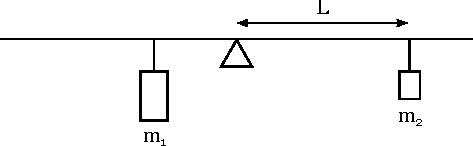
\includegraphics[]{./lab6_part1.pdf}
\end{center}
\end{figure}

Make a graph of position ($y$-axis) versus 1/weight ($x$-axis) of $m_2$ and find a best-fit relationship between position and weight. \textbf{Note that you need to account for the mass of the brackets when calculating weights.} Explain your results and compare with what you expected to find. What is the meaning of the slope? What about the y-intercept? Include the graph in your lab report. Be sure to use proper units and to label the axes.

\vspace{.5cm}

\renewcommand{\arraystretch}{1.4}
\newcolumntype{Y}{>{\centering\arraybackslash}X}
\begin{tabularx}{\linewidth}{|Y|Y|Y|Y|}
\hline
\vspace{2cm} & mass, $m_2$ & weight, $\left(F_g\right)_2$ & distance, $L$ \\
\hline Trial 1 &&&\\
\hline Trial 2 &&&\\
\hline Trial 3 &&&\\
\hline Trial 4 &&&\\
\hline Trial 5 &&&\\
\hline
\end{tabularx}\\

Use Newton's Laws to find a theoretical relationship between the distance $L$ and the weight ($F_g$) of $m_2$. In other words, set $\sum\tau=0$ and solve for $L$. How does this relationship compare to your graph?


\section{MASS OF THE METER STICK}
(a) Gravitational forces can be treated as acting at the center of the mass of an object. Using this concept, you will compute the mass of the meter stick by solving a static equilibrium problem. Set up an arrangement of parallel (vertical) forces by placing the fulcrum anywhere other than the center of mass of the meter stick. By placing appropriate masses as shown in the diagram, make the meter stick balance.  What is the mass of the meter stick?

\begin{figure}[h]
\begin{center}
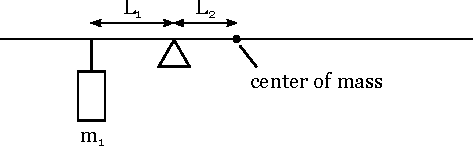
\includegraphics{./lab6_part2a.pdf}
\end{center}
\end{figure}

Repeat the experiment with different values of $m_1$, $L_1$, and $L_2$ to confirm the value of the meter stick's mass that you found.
 
\begin{tabularx}{\linewidth}{|Y|Y|Y|Y|}
\hline
mass, $m_1$ & $L_1$ & $L_2$ & meter stick mass \\
\hline &&&\\
\hline &&&\\
\hline &&&\\
\hline &&&\\
\hline
\end{tabularx}\\

Be sure to demonstrate how you calculated the mass of the meter stick. Use a scale to measure the mass of the meter stick to compare to your calculations.

\clearpage
(b) With an unequal arm balance, such as shown in the diagram below, hang
a mass on each side of the meter stick in such a way to make it
balance.  (That is, using a rotation point that is not at the center
of mass of the meter stick, use two masses and find the balance
points.)  Record the masses and distances and compare them to a
calculation of the situation you have created.

\begin{figure}[h]
\begin{center}
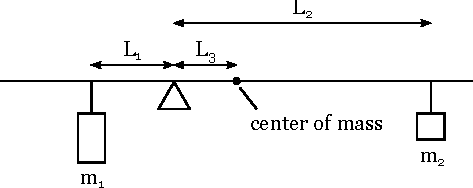
\includegraphics{./lab6_part2b.pdf}
\end{center}
\end{figure}

\begin{tabularx}{\linewidth}{|Y|Y|Y|Y|Y|}
\hline
$m_1$ & $m_2$ & $L_1$ & $L_2$ & $L_3$\\
\hline &&&&\\
\hline &&&&\\
\hline &&&&\\
\hline
\end{tabularx}\\

One way to compare your measurements to theory is to solve for $L_2$ using $\sum\tau=0$. Show how you do this and compare the theoretical values of $L_2$ to what you measured.

How much would your theoretical values of $L_2$ have differed from the experimental values if you had neglected to account for the mass of the meter stick in your derivation?

\section{MASS OF HANGING SPHERE}
Hang the metal sphere from two strings that are connected to the tension protractors. The strings should not be vertical.
\begin{figure}[h]
  \begin{center}
    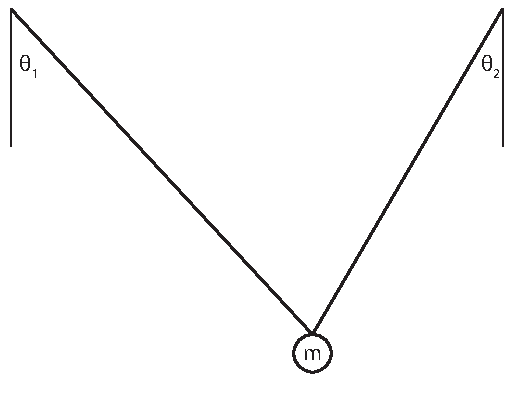
\includegraphics[]{./hanging_mass.pdf}
  \end{center}
\end{figure}

Determine the mass of the sphere by measuring the forces and angles from the tension protractors and applying Newton's Laws.

What would the initial angular acceleration be if one of the strings was cut? The moment of inertia of a sphere rotating around some point axis is $I=m\left(d^2+\frac{2}{5}r^2\right)$, where $r$ is the radius of the sphere and $d$ is the distance from the center of the sphere to the axis of rotation. How much different would your answer be if you assumed that the sphere was a point mass, in which case the moment of inertia would be $I=md^2$?

\end{document}
